

\section{Introduction}
Over the years, various research demonstrated the impact of web design on how user's find content on the web\cite{nielsen1999designing}\cite{nielsen2006f}\cite{pernice2017f}.  Although web design has become a 34 billion dollar industry in the US alone according to \citet{ibisdesign}, modern search engines are still focused on using content features (e.g., BM25, pagerank and clickthrough ratio) to determine web relevance. 
% Although these design principles have been widely adopted in the field of web design, modern search engines are still focused on using content features for document relevance. 
% According to \citet{ibisdesign}, the US web design industry alone had an annual revenue of approximately 34 billion dollar in 2017. 

Recently \citet{fan2017learning} introduced ViP, a learning to rank (LTR) model that uses a combination of both visual and content features. Visual features are represented as screenshots created by rendering the available webpages. The authors demonstrate that adding these screenshots significantly improve LTR performance. The indication that the visual representation of a web page can have a significant improvement on web search, leverages a new field in LTR research. 
However, the .GOV2 collection that is used for rendering webpages is limited by the fact that: i) it solely contains pages within the .gov domain from 2002, ii) images are not included, iii) styling is relatively simple. Considering these limitations, further visual LTR research should use a more diverse out-of-the-box retrieval dataset with judgments, content features and screenshots. 

In this work, we propose \datasetname, a dataset that allows the LTR research community to investigate various methods of using Visual Features in web relevance. \datasetname is a combination of queries \& content features from TREC Web 2013 \& 2014 and screenshots from ClueWeb12 documents. 

Using \datasetname we showed that the results from \citet{fan2017learning} can be reproduced on a more diverse dataset. Moreover, we demonstrated that by applying transfer learning from a pre-trained image recognition model we were able to make a significant improvement in retrieval performance. 

The main contribution of this work are:
\begin{enumerate}  
\item A demonstration of the abilities of visual features in LTR.
\item An out-of-the-box dataset for visual LTR research.
\item A baseline for future visual LTR research.
\end{enumerate}

Section \ref{sec:dataset} describes the collection process that was used to construct \datasetname. In section \ref{sec:experiments} we reproduce the work of \citet{fan2017learning}, demonstrate various feature extraction methods on \datasetname and set a baseline for future visual LTR research.  


% \begin{itemize}[noitemsep]
% \item Can we construct a dataset that can be used for experiments on visual features for Learning To Rank.
% \end{itemize}

\section{Related work}\label{sec:relatedwork}
The work of \citet{nielsen1999designing} argues that when the design has not been well performed, a user searching for information is easily diverted to a competitors website. More recent work by \citet{nielsen2006f} and \citet{pernice2017f} use eye tracking equipment to demonstrate how different design patterns influences the search patterns of various users.


\section{Dataset}\label{sec:dataset}
In this section, we explain the collection process of the \datasetname dataset. Subsection \ref{sec:trecclue} contains more information about the underlying TREC WEB query sets and ClueWeb12 document collection. Details on how the content features are calculated using Apache Spark is discussed in subsection \ref{sec:contentfeature}. The collection of screenshot from the ClueWeb12 collection using the Wayback Machine and ClueWeb12 Online rendering service is explained in subsection \ref{sec:screenshotsec}. Finally, subsection \ref{sec:datasetsum} gives an overview of the structure in which the full collection is presented.

\subsection{TREC Web \& ClueWeb12 }\label{sec:trecclue}
\datasetname uses query sets TREC Web 2013~\cite{collins2013trec} \& 2014~\cite{collins2015trec}. Table \ref{tab:webstats} contains a detailed description of the amount of queries and relevance labels in both TREC web query sets.

\begin{center}
  \begin{tabular}{ l | c | c | c }
    measure & TREC WEB 2013 & TREC WEB 2014 \\
    \hline
    Total documents & 14,474 & 14,432 \\
    Queries & 50 & 50 \\
    Nav grade (4) & 7 & 33 \\
    Key grade (3) & 179 & 230 \\
    Hrel grade (2) & 1154 & 2168 \\
    Rel grade (1) & 3044 & 3788 \\
    Non grade (0) & 10090 & 8210 \\
    Junk grade (-2) & 234 & 554 \\
    \hline
  \end{tabular}
  \captionof{table}{Document and relevance labels in TREC web 2013 \& 2014.} \label{tab:webstats} 
\end{center}

Both TREC web query sets have been judged on documents from the  ClueWeb12\footnote{\url{https://lemurproject.org/clueweb12/}} collection, which is an unfiltered and highly diverse collection of web pages scraped in the first half of 2012. The total collection contains well over 700 million documents that are crawled using the typical crawling settings of Heritrix archival crawler project\footnote{https://webarchive.jira.com/wiki/spaces/Heritrix/overview} from archive.org.  


\begin{table*}[t]
\begin{center}
\begin{tabular}{llllllll}
\multicolumn{8}{c}{MQ2007 46 features}                                     \\
           & P@1    & P@5    & P@10   & NDCG@1 & NDCG@5 & NDCG@10 & MAP    \\ \hline
RankBoost  & 0.453 & 0.404 & 0.371 & 0.391 & 0.403 & 0.430  & 0.457 \\
AdaRank    & 0.420 & 0.402 & 0.360 & 0.367 & 0.403 & 0.424  & 0.449 \\
LambdaMart & 0.452 & 0.418 & 0.384 & 0.405 & 0.411 & 0.444  & 0.463 \\
\hline
\\
\end{tabular}
\\
\begin{tabular}{llllllll}
\multicolumn{8}{c}{MQ2007 11 features}                                 \\
           & P@1   & P@5   & P@10  & NDCG@1 & NDCG@5 & NDCG@10 & MAP   \\ \hline
RankBoost  & 0.448 & 0.400 & 0.372 & 0.381  & 0.401  & 0.431   & 0.453 \\
AdaRank    & 0.385 & 0.391 & 0.287 & 0.364  & 0.396  & 0.394   & 0.386 \\
LambdaMart & 0.448 & 0.412 & 0.380 & 0.397  & 0.411  & 0.443   & 0.455 \\
\hline
\\
\end{tabular}
\captionof{table}{A benchmark comparison between the MQ2007 query set using all 46 LETOR features and the 11 LETOR features that are used in \datasetname.}\label{tab:11vs46}
\end{center}
\end{table*}



% Insert WEB & CLUEWEB statistics.
\subsection{Content features} \label{sec:contentfeature}
The content features were collected in a full pass over the complete ClueWeb12 with Apache Spark using 116 Hadoop worker nodes with 3 executor cores and 21gb memory each. A HTML parser (jsoup\footnote{https://jsoup.org/}) was used to create separate items for the title and content from the raw HTML. Because the HTML structure of some of the larger documents could not be parsed by jsoup, all documents with more than one million terms were ignored. Using the Apache Spark 2.2.1 implementation of TF and IDF, a sparse vector was obtained for each item in each document.  On top of the IR features, PageRank scores from the ClueWeb12 \textit{Related Data} section\footnote{https://lemurproject.org/clueweb12/related-data.php} were added to each document as well. A full overview of all computed content features can be found in table \ref{tab:setdescription}. Finally, the following modifications based on the features from LETOR 3.0 \cite{qin2010letor} were made to stabilize training.
\begin{enumerate}  
% \item IDF is calculates as follows: 
% $$IDF(q, D) = \sum_{t_i \in q} IDF(t_i, D) = \sum_{t_i \in t} \log \frac{|D| + 1}{DF(t_i) + 1}$$
% Where  $q_i$ and $t_i$ represent a list of all terms in a query and a single query term respectively. $D$ represents a list of all terms in a document with $|D|$ as its total length. $DF(t_i)$ is the document frequency for the given query term.  
\item Free parameters $k_1$, $k_3$ and $b$ for BM25 were set to $2.5$, $0$ and $0.8$ respectively. 
\item Because the PageRank score are usually an order of magnitude smaller than all the other scores, we multiplied each value with $10^5$.
\item After all features have been computed, the log is taken over the final results.
\item The logged features are normalized per query.  
\end{enumerate}


 
\begin{center}
\centering
\label{my-label}
\begin{tabular}{ll}
Id & Description    \\ \hline
1  & Pagerank       \\
2  & Content length \\
3  & Content TF     \\
4  & Content IDF    \\
5  & Content TFIDF  \\
6  & Content BM25   \\
7  & Title length   \\
8  & Title TF       \\
9  & Title IDF      \\
10 & Title TFIDF    \\
11 & Title BM25    
\end{tabular}
\captionof{table}{A description of all content features provided with \datasetname1.}  \label{tab:setdescription} 
\end{center}



%\textit{(This has not been done yet)} The TF and IDF scores were also calculated Anchor text extracted by \citet{hiemstra2010mapreduce} 
% Make a seperate section for screenshots and subsections for collection, cleaning, statistics etc.

\subsection{Screenshots} \label{sec:screenshotsec}

\begin{table*}[t]
\begin{center}
\begin{tabular}{llllllll}
\multicolumn{8}{c}{Clueweb12 11 features}                                    \\ 
                      & P@1   & P@5   & P@10  & NDCG@1 & NDCG@5 & NDCG@10 & MAP   \\ \hline
RankBoost             & 0,460 & 0,432 & 0,420 & 0,184  & 0,212  & 0,233   & 0,426 \\
AdaRank               & 0,310 & 0,376 & 0,335 & 0,135  & 0,133  & 0,150   & 0,344 \\
LambdaMart            & 0,370 & 0,480 & 0,477 & 0,145  & 0,238  & 0,247   & 0,438 \\ \hline
ViP baseline          & 0,348 & 0,371 & 0,385 & 0,186  & 0,221  & 0,241   & 0,414 \\ \hline
ViP masks             & 0,346 & 0,391 & 0,399 & 0,186  & 0,232  & 0,251   & 0,419 \\
ViP highlights        & 0,394 & 0,404 & 0,424 & 0,220  & 0,242  & 0,264   & 0,422 \\
ViP snapshots         & 0,354 & 0,364 & 0,387 & 0,196  & 0,218  & 0,242   & 0,420 \\ \hline
VGG-16 snapshots      & 0,514 & 0,488 & 0,484 & 0,292  & 0,307  & 0,324   & 0,442 \\ \hline
\end{tabular}
\centering
\captionof{table}{Results after 5 iterations on all 5 folds of \datasetname. ViP is the model by \citet{fan2017learning}, the baseline uses only content features and VGG-16 is the pre-trained feature extractor.}
\label{tab:results}
\end{center}
\end{table*}


\subsubsection{Collection}
Although each entry in the ClueWeb12 collection contains the full HTML, many pages lack the required styling and images files in order to render the full page. Instead, we used the Wayback Machine\footnote{http://archive.org/web/} from Archive.org which offers various archived versions of webpages since 2005. Other than the archive in ClueWeb12, the Wayback Machine also offers styling and images for each webpage. Scraping was performed on the available entry on Wayback that is closest to the original scrape data. A screenshot is then taken using a headless instance of the Firefox browser together with the Python implementation of the Selenium testing framework. 
For reproduction of the work from \citet{fan2017learning}, two separate datasets of images are available containing screenshots with red highlighted query words and the query word locations as a black mask on a white background. 

\begin{figure}[h]
\begin{tabular}{ccc}
\subfloat{
\includegraphics[width = 1in]{images/1-snapshot.png}} &
\subfloat{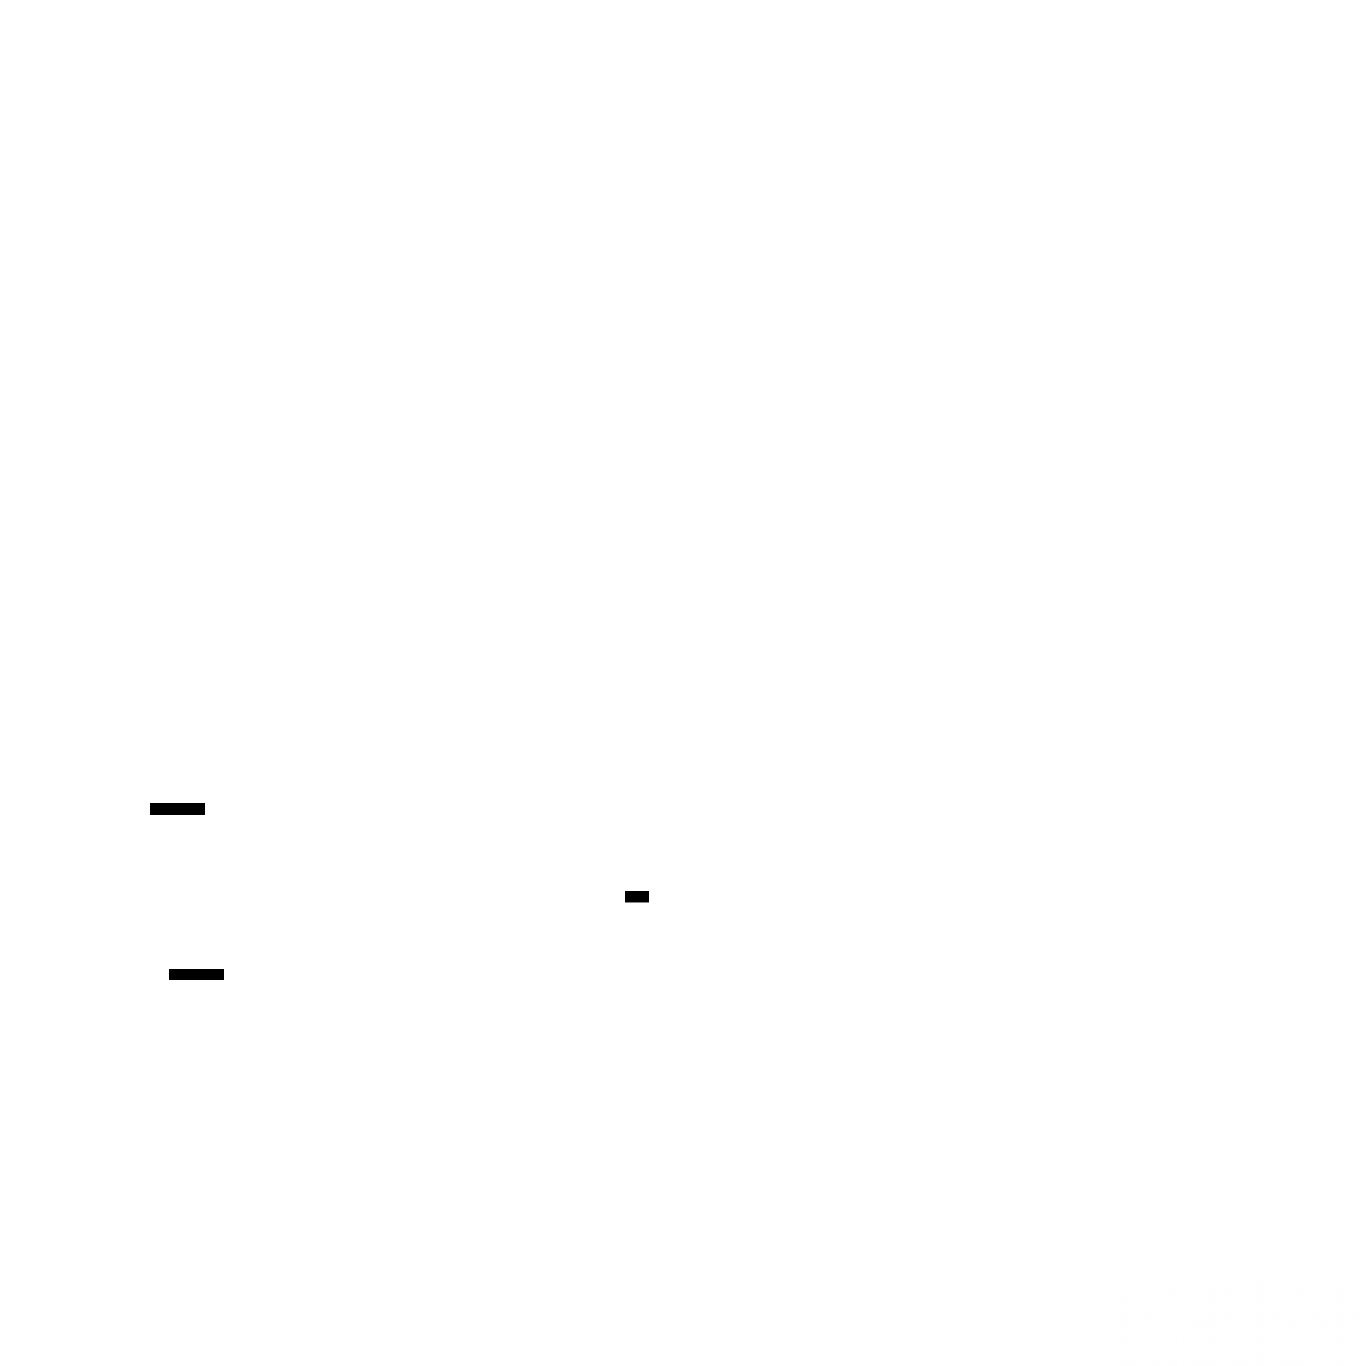
\includegraphics[width = 1in]{images/1-mask.png}} &
\subfloat{
\includegraphics[width = 1in]{images/1-highlights.png}}\\
\subfloat{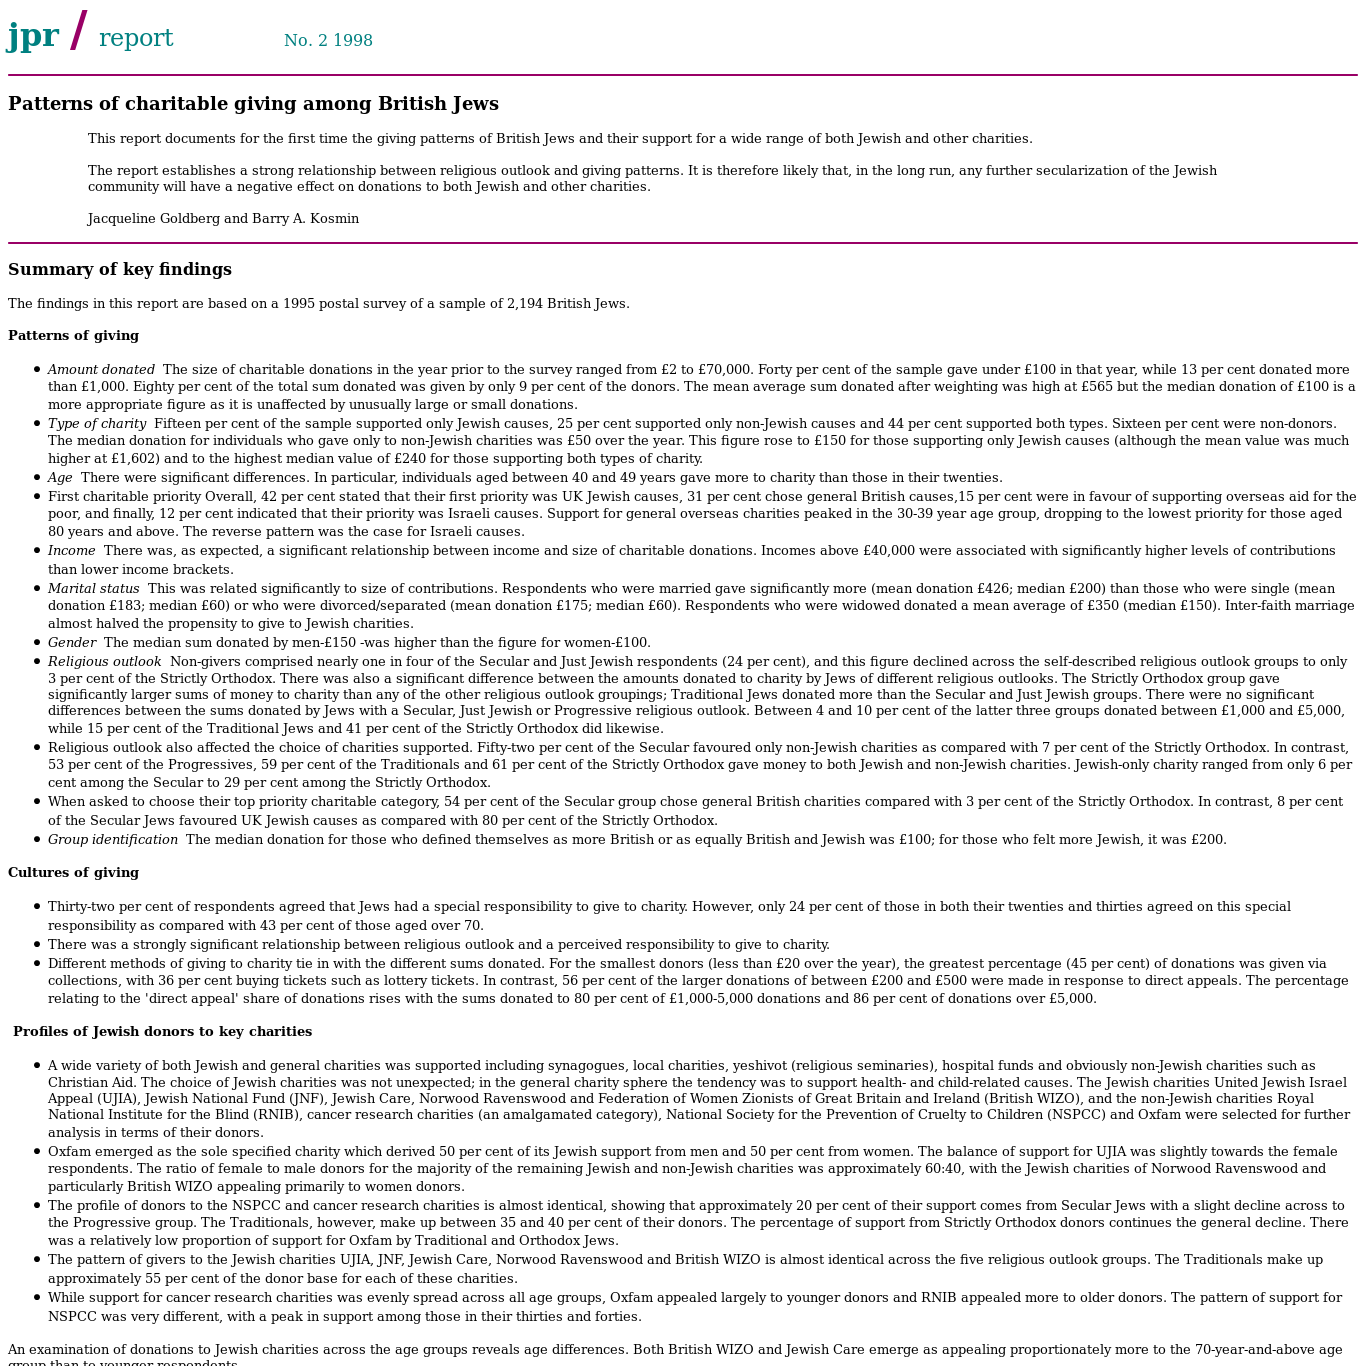
\includegraphics[width = 1in]{images/2-snapshot.png}} &
\subfloat{
\includegraphics[width = 1in]{images/2-mask.png}} &
\subfloat{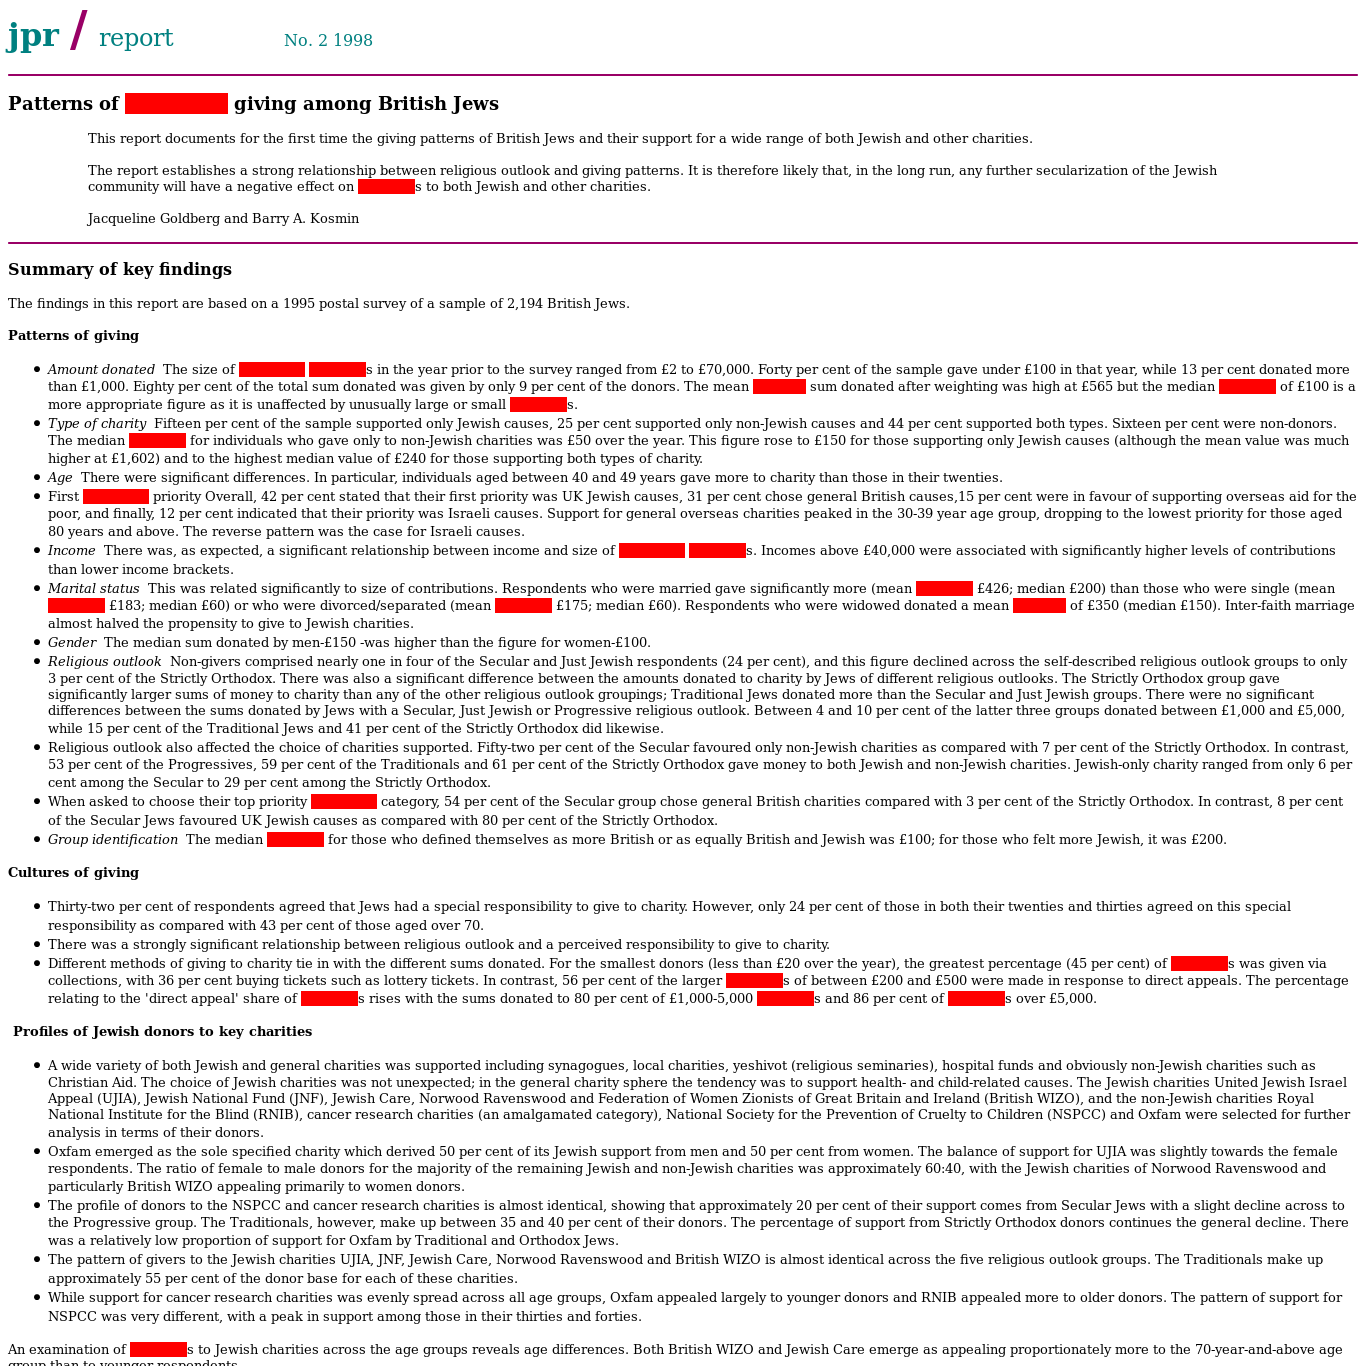
\includegraphics[width = 1in]{images/2-highlights.png}}\\
\subfloat{
\includegraphics[width = 1in]{images/3-snapshot.png}} &
\subfloat{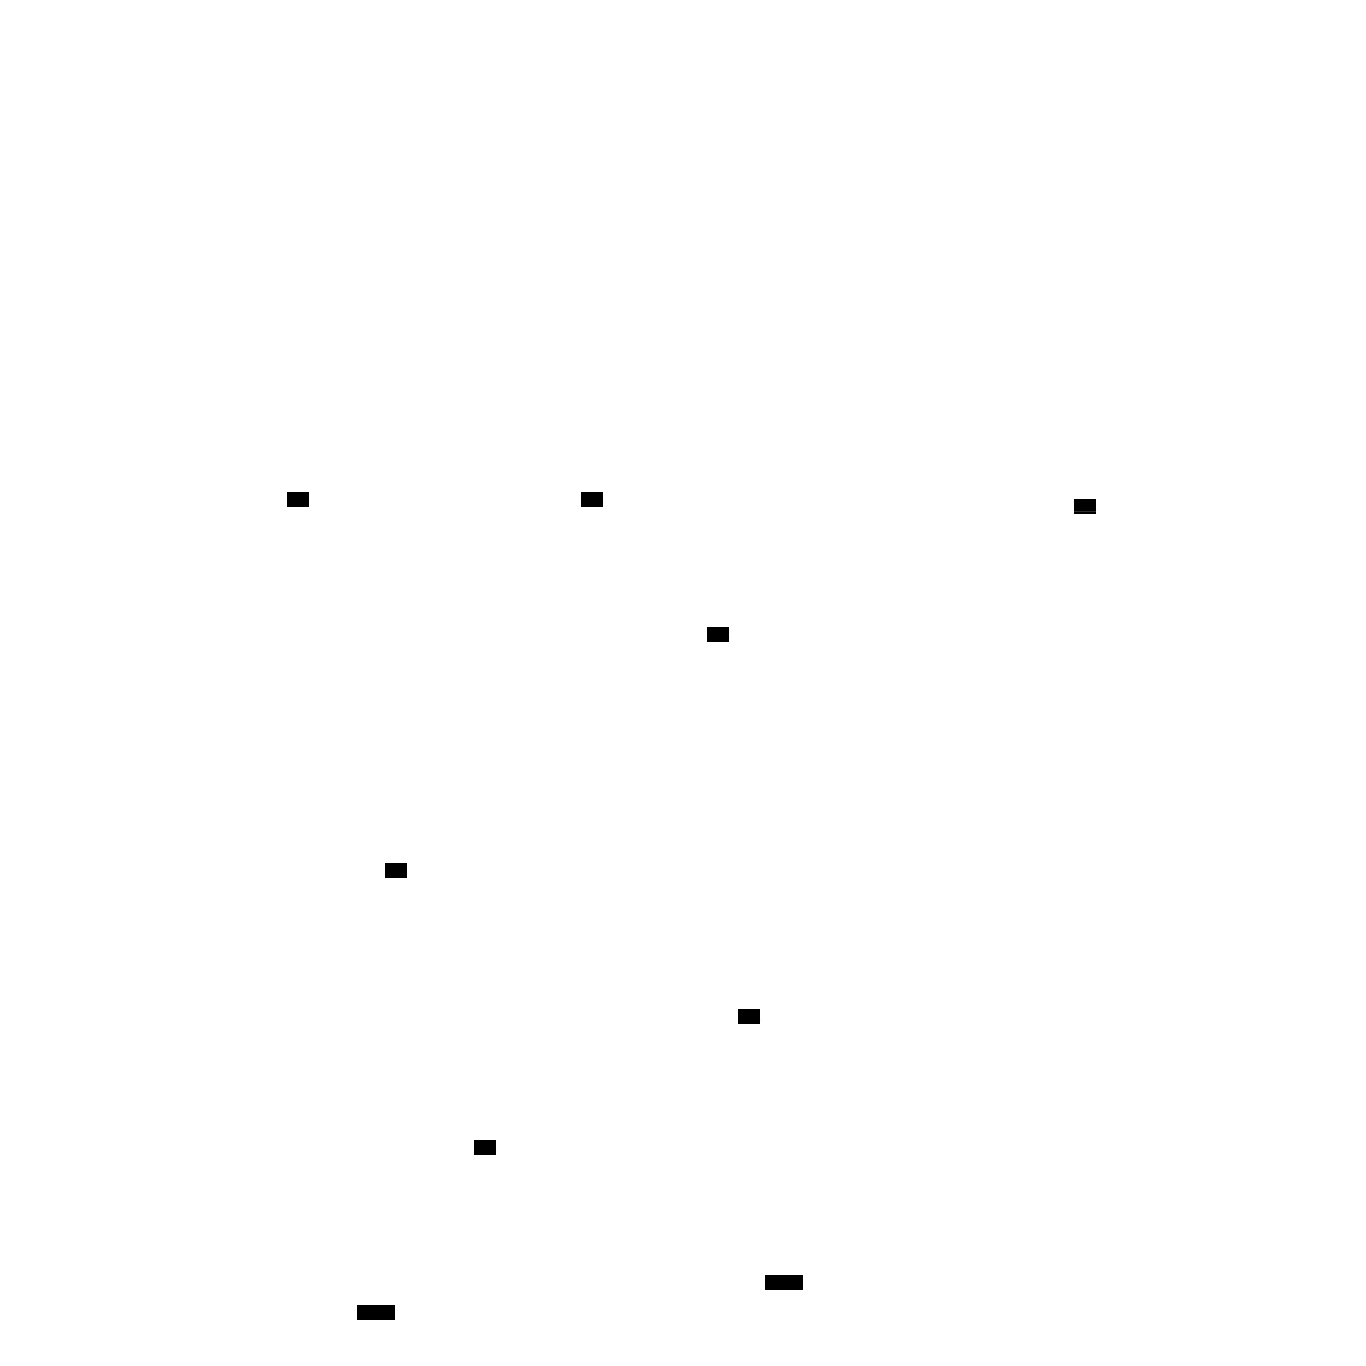
\includegraphics[width = 1in]{images/3-mask.png}} &
\subfloat{
\includegraphics[width = 1in]{images/3-highlights.png}}\\
\end{tabular}
\caption{Examples of the vanilla screenshot, mask and red highlighted screenshot from left to right respectively}
\end{figure}

\subsubsection{Filtering}\label{sec:datasetsum}
As the Wayback Machine does not contain an archived version of each document in the ClueWeb12 collection, some filtering was required in order to increase the overall quality of the screenshots. The following criteria were used in order to get a screenshot for each document.
\begin{enumerate}    
\item Each document was requested from the Wayback Machine separately. 
\item Documents that were not on the Wayback Machine, timed out, threw a JavaScript error or resulted in a .PNG screenshot smaller than 100kb are rendered using the ClueWeb12 online rendering service.
\item A manual selection was made between all documents that were in both sets: The Wayback version was used if this contained styling and the content was the same as the rendering service. Otherwise, the rendering service version was used.
\end{enumerate}

\begin{table}[h]
  \begin{tabular}{ l | c | c  }
    score & Wayback Machine & ClueWeb12 \\
    \hline
    Total & 22825 & 6081 \\
    Nav grade (4) & 33 & 5 \\
    Key grade (3) & 336 & 34 \\
    Hrel grade (2) & 2209 & 148 \\
    Rel grade (1) & 5589 & 502 \\
    Non grade (0) & 14119 & 5227 \\
    Junk grade (-2) & 539 & 165 \\
    \hline
  \end{tabular}
  \captionof{table}{The amount of documents with a screenshot from the Wayback Machine and from ClueWeb12, including their relevance score. (Note: This table is not up to date)} \label{tab:countsources} 
\end{table}

At the end of the process, each judged document has a corresponding screenshot from either the Wayback Machine or ClueWeb12 rendering service. Table \ref{tab:countsources} shows how the different sources are divided.

\subsection{Final collection}
All results mentioned in the previous subsections are delivered in three components. The TREC WEB queries and content features are combined into three LETOR formatted files with the raw, logged and query normalized values. The query normalized files is separated in 5 fold-partitions containing 20 queries each. Each of the 5 folds contains a training file from three fold-partitions with the other two fold-partitions being the test and training files. A separate file containing the quality scores can be used to filter which documents to use for training. Each screenshot is stored as a .PNG and can be identified by their corresponding ClueWeb12 name. 

\begin{figure*}[t]
\centering
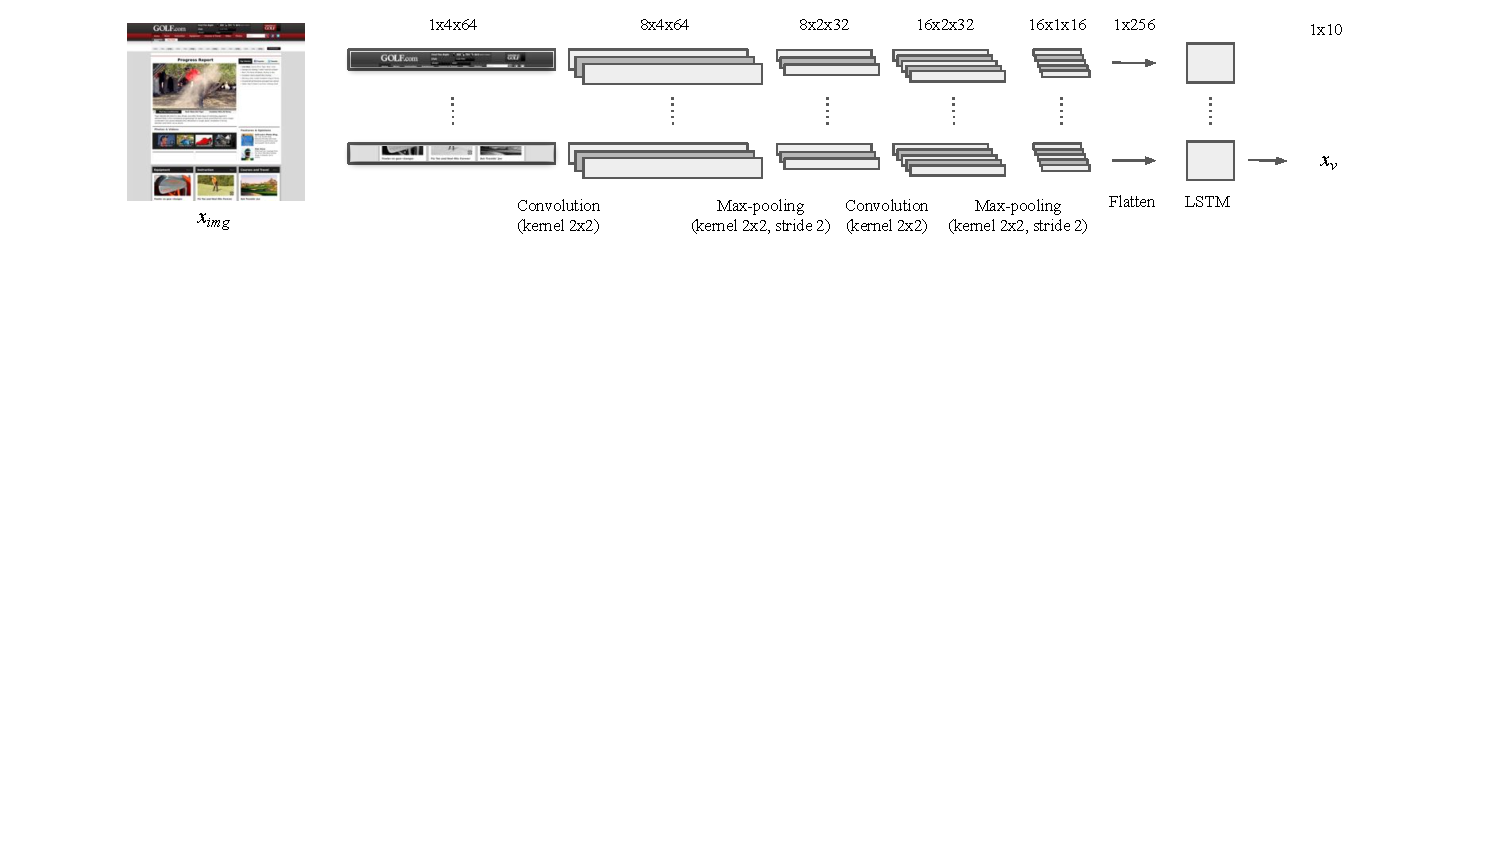
\includegraphics[clip,trim=0 10cm 0 0, width=20cm]{images/vip-features.pdf}
  \captionof{figure}{The feature extractor architecture with corresponding dimensions used in our implementation of the ViP model.} \label{fig:ViPfeat} 
\end{figure*}

\section{Experimental Setup}\label{sec:experiments}
In this section, we discuss the experiments performed on \datasetname. 
%All PyTorch experiments were performed on a GTX 1080 Ti with 11gb of RAM. Preproccessing was performed on a Thinkpad X250 with an Intel i5-5300U CPU and 16gb of ram. 


\subsection{Benchmarking content features}
The quality and performance of the computed content features are benchmarked against the MQ2007 query set using content features from LETOR 4.0. The implementations of RankBoost, AdaRank and LambdaMart from RankLib\footnote{https://sourceforge.net/p/lemur/wiki/RankLib/} with their default settings were used for the experiments. Table \ref{tab:11vs46} shows the difference in performance between the MQ2007 LETOR 4.0 features, our WEB track features and MQ2007 using the same 11 features used for the WEB track. Each entry has been separately trained and optimized in 5 folds on the corresponding evaluation method. 

\subsection{Visual feature models}
In order to work with the visual features, we use a base structure by \citet{fan2017learning} where the model is split into a visual feature extraction and scoring component. The visual feature extraction component takes image $x_{img}$ as an input and outputs visual feature vector $x_{v}$. This feature vector concatenated with content feature vector $x_{c}$ is used as input to the scoring component. In our case the scoring component is a simple fully connected layer with a hidden size of $10$ with dropout of $.1$. The combined models are trained end-to-end using pairwise hinge loss with $l_2$ regularization. 

For the experiments, we used various feature extraction models and image inputs which are both described below.


\subsubsection{ViP visual features}
As a baseline, we implemented the visual feature extractor proposed by \citet{fan2017learning} in PyTorch. In this model, the input image is gray-scaled and segmented into $4x16$ slices which are processed separately through a shallow convolutional network. This output is then passed top to bottom through a LSTM which results in the final visual feature vector. The full dimensions can be found in figure \ref{fig:ViPfeat}.

\subsubsection{VGG-16 visual features}
Because \datasetname has a relatively low amount of image to train on, we use an on ImageNet pretrained VGG-16 \cite{simonyan2014very} as visual feature extractor. The last fully connected layer is replaced by a layer with an output of size $30$, with weights initialized  During training, we update the weights in all fully connected layer and keep the convolutional layers fixed. Other than the ViP feature extractor, VGG-16 uses a $224x224$ image with three color channels as input. 

\subsubsection{Image inputs}
In this work we use three types of image inputs during training. 
% TODO: Write something amount how the three image input are constructed and relevant

\section{Results}
\section{Acknowledgements}
The Spark experiments in this work were carried out on the Dutch national e-infrastructure with the support of SURF Cooperative. Thanks to the Amsterdam Robotics Lab for using their computational resources. Thanks to Jamie Callan and his team for providing access to the online services for ClueWeb12. 
